\chapter{Related Work}

The study of urban spatial order, street network structures, and scene uniqueness
has been explored for several decades. Early research in urban planning and geography
laid the groundwork for understanding how street networks shape human interaction and movement.
Over time, researchers have developed methods to classify urban layouts, analyze spatial
entropy, and quantify scene distinctiveness.

By looking at foundational works from the mid-20th century and comparing them with modern
methodologies, we can see that while general urban
morphology has been well studied, the specific topic of scene uniqueness and distinctiveness in spatial networks
is an emerging area with room for further exploration.

\section{Urban Spatial Order and Street Network Typologies}
Early research on street networks can be traced back to studies in urban morphology and
planning, such as by \citet{Lynch1960}. Lynch introduced the concept of imageability,
where certain urban features stand out as recognizable reference points, a concept closely
tied to scene uniqueness.
\begin{figure}[!htb]
    \begin{minipage}{0.52\textwidth}
        \centering
        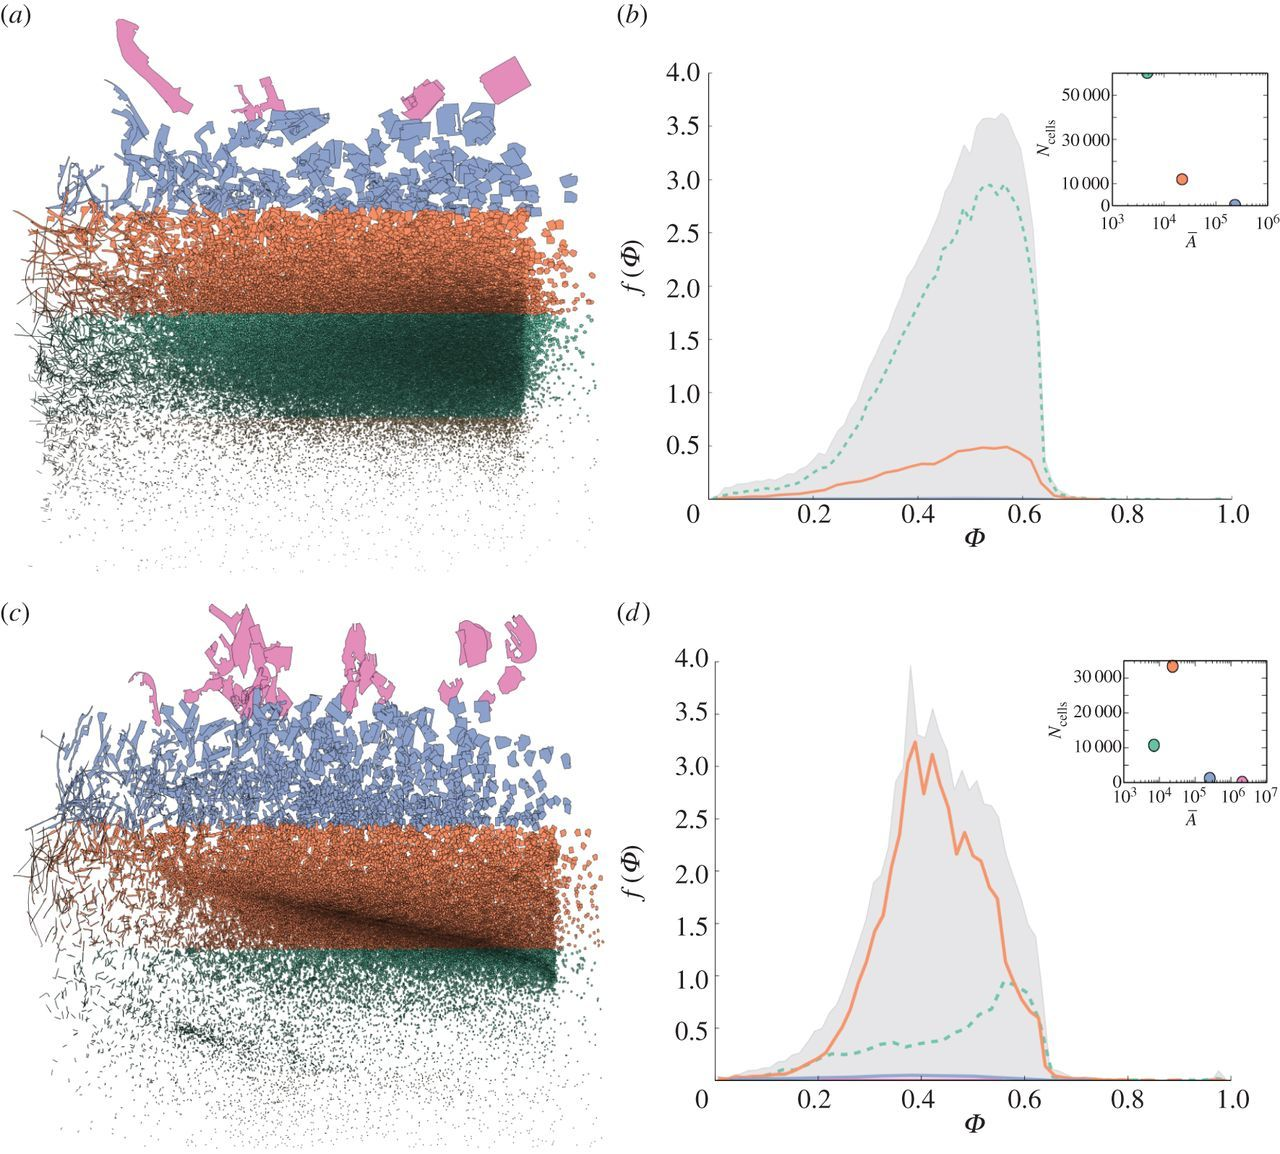
\includegraphics[width=.7\linewidth]{../fingerprints_Tokyo_NewYork.png}
        \caption{The fingerprints of Tokyo (a,b) and New York, NY (c,d). (a,c) from \citet{remi_2014}}
    \label{fig:fingerprints_tokyo_newyork}
    \end{minipage}\hfill
    \begin{minipage}{0.48\textwidth}
        \centering
        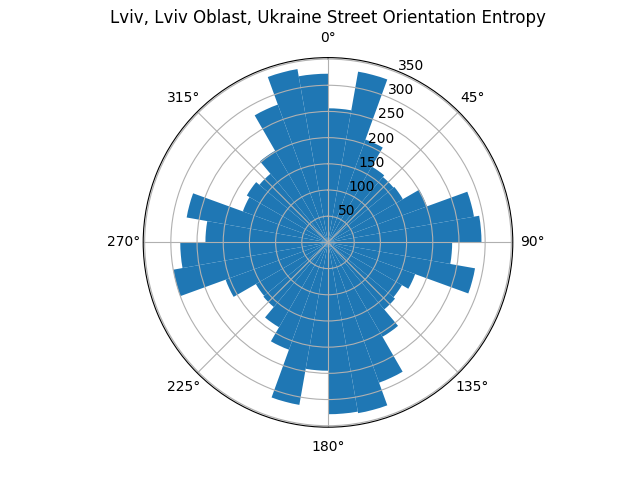
\includegraphics[width=.7\linewidth]{../street_orientation_entropy_LvivLvivOblastUkraine.png}
        \caption{Street orientation entropy for Lviv, Lviv Oblast, Ukraine.}
        \label{fig:street_orientation_entropy}
    \end{minipage}
\end{figure}
Building on these ideas, \citet{remi_2014} developed a typology of street patterns, showing how
different cities exhibit unique structural characteristics. Their clustering approach classified
cities into distinct groups based on the shape and distribution of urban blocks. This work provides
a framework for understanding how spatial arrangements contribute to distinctiveness
but does not directly focus on scene recognizability.

One of the major studies in this domain is \textit{Urban spatial order: street network orientation,
configuration, and entropy} by \citet{Boeing_2019}, which investigates the
orientation, configuration, and entropy of street networks across 100 cities worldwide
using OpenStreetMap (OSM) \cite{OpenStreetMap} data and the OSMnx \cite{osmnx} toolkit. Boeing uses orientation entropy to
measure the degrees of order and disorder in urban layouts, finding that American cities tend to be
highly ordered while European cities exhibit higher entropy due to organic growth patterns - Figures \ref{fig:polar_histograms} and \ref{fig:street_orientation_entropy}.
However, his research also does not extend to how these patterns contribute to geospatial
distinctiveness from a navigational perspective.

We can see the street orientation entropy for Lviv, Lviv Oblast, Ukraine, calculated
using the methodology proposed by \citet{Boeing_2019} in Figure \ref{fig:street_orientation_entropy}.,
and preliminary data for the future analysis of urban scene uniqueness in Lviv, Lviv Oblast, Ukraine and Manhattan, New York, USA in Figures \ref{fig:urban_analysis_metrics} and \ref{fig:urban_analysis_metrics_manhattan}

\begin{figure}[!htb]
    \centering
    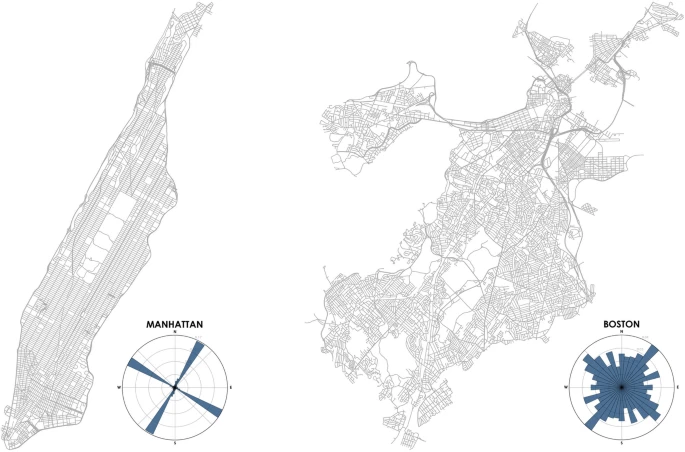
\includegraphics[width=0.8\textwidth]{../polar_histograms_ManhattanBoston.png}
    \caption{Street networks and corresponding polar histograms for Manhattan and Boston. \citet{Boeing_2019}}
    \label{fig:polar_histograms}
\end{figure}

\begin{figure}[!htb]
    \centering
    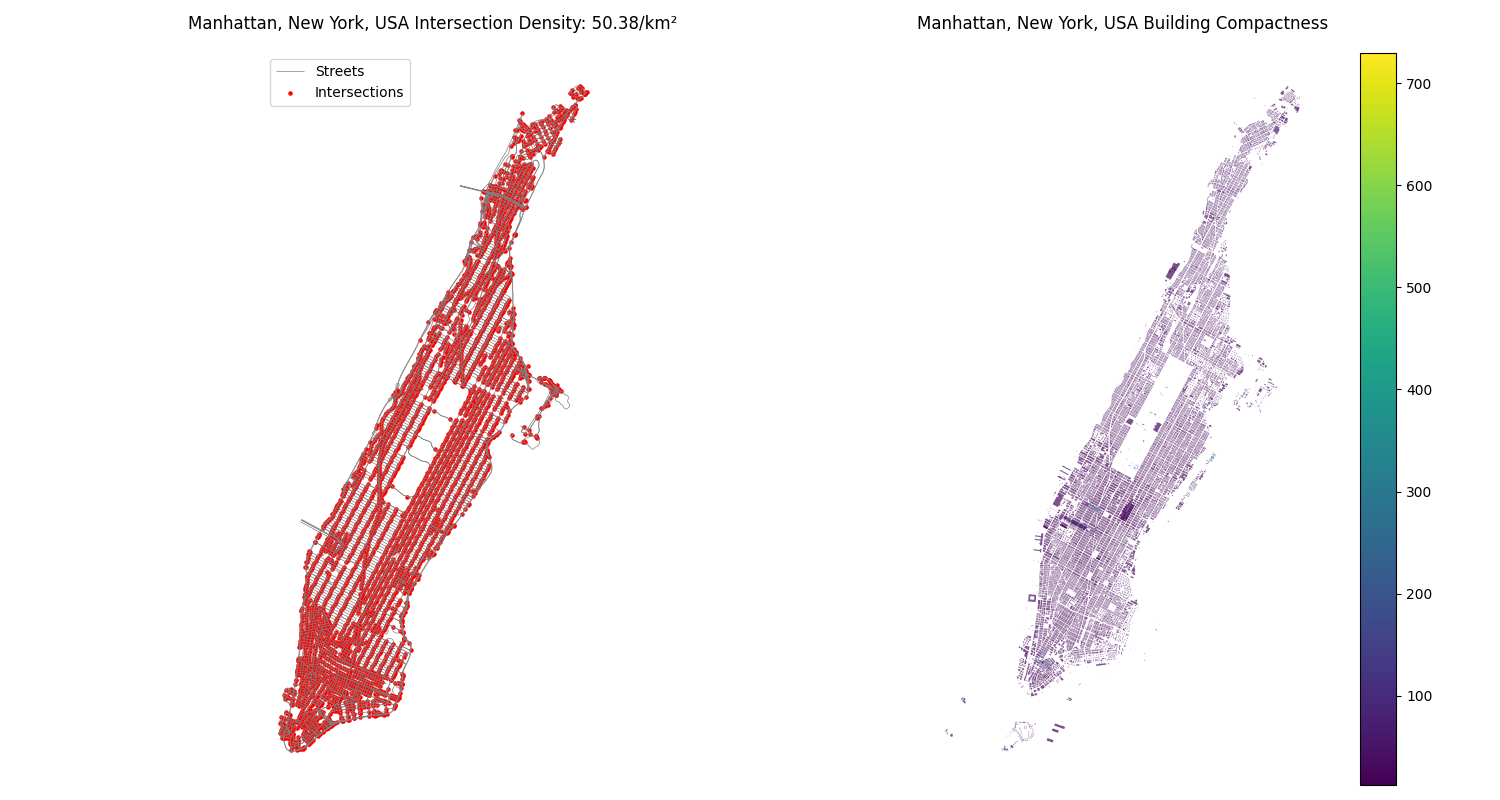
\includegraphics[width=0.8\textwidth]{../urban_analysis_metrics_ManhattanNewYorkUSA.png}
    \caption{Urban analysis metrics for Manhattan, New York, USA.}
    \label{fig:urban_analysis_metrics_manhattan}
\end{figure}

\begin{figure}[!htb]
    \centering
    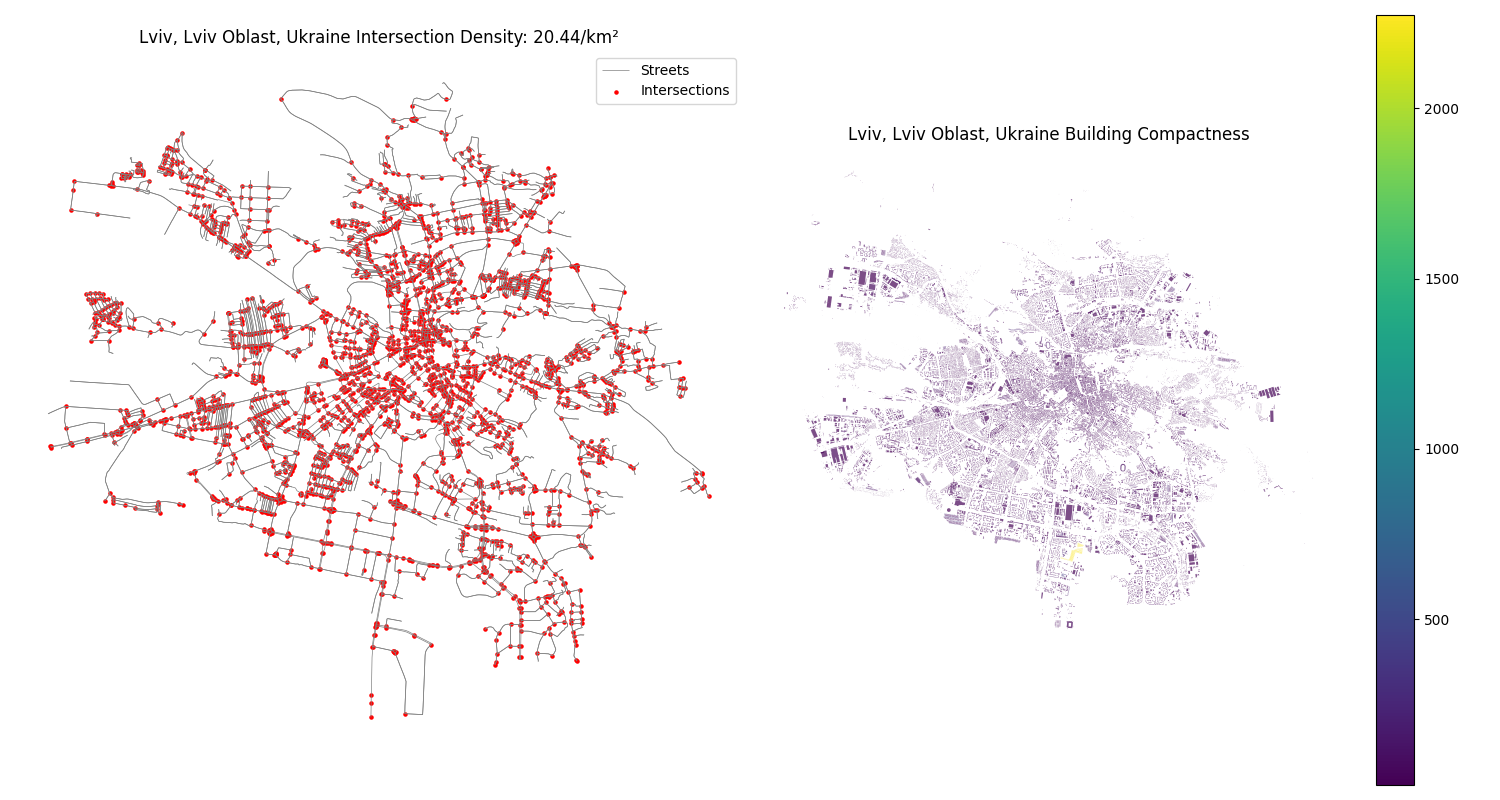
\includegraphics[width=0.8\textwidth]{../urban_analysis_metrics_LvivLvivOblastUkraine.png}
    \caption{Urban analysis metrics for Lviv, Lviv Oblast, Ukraine.}
    \label{fig:urban_analysis_metrics}
\end{figure}

\begin{figure}[h!tb]
    \centering
    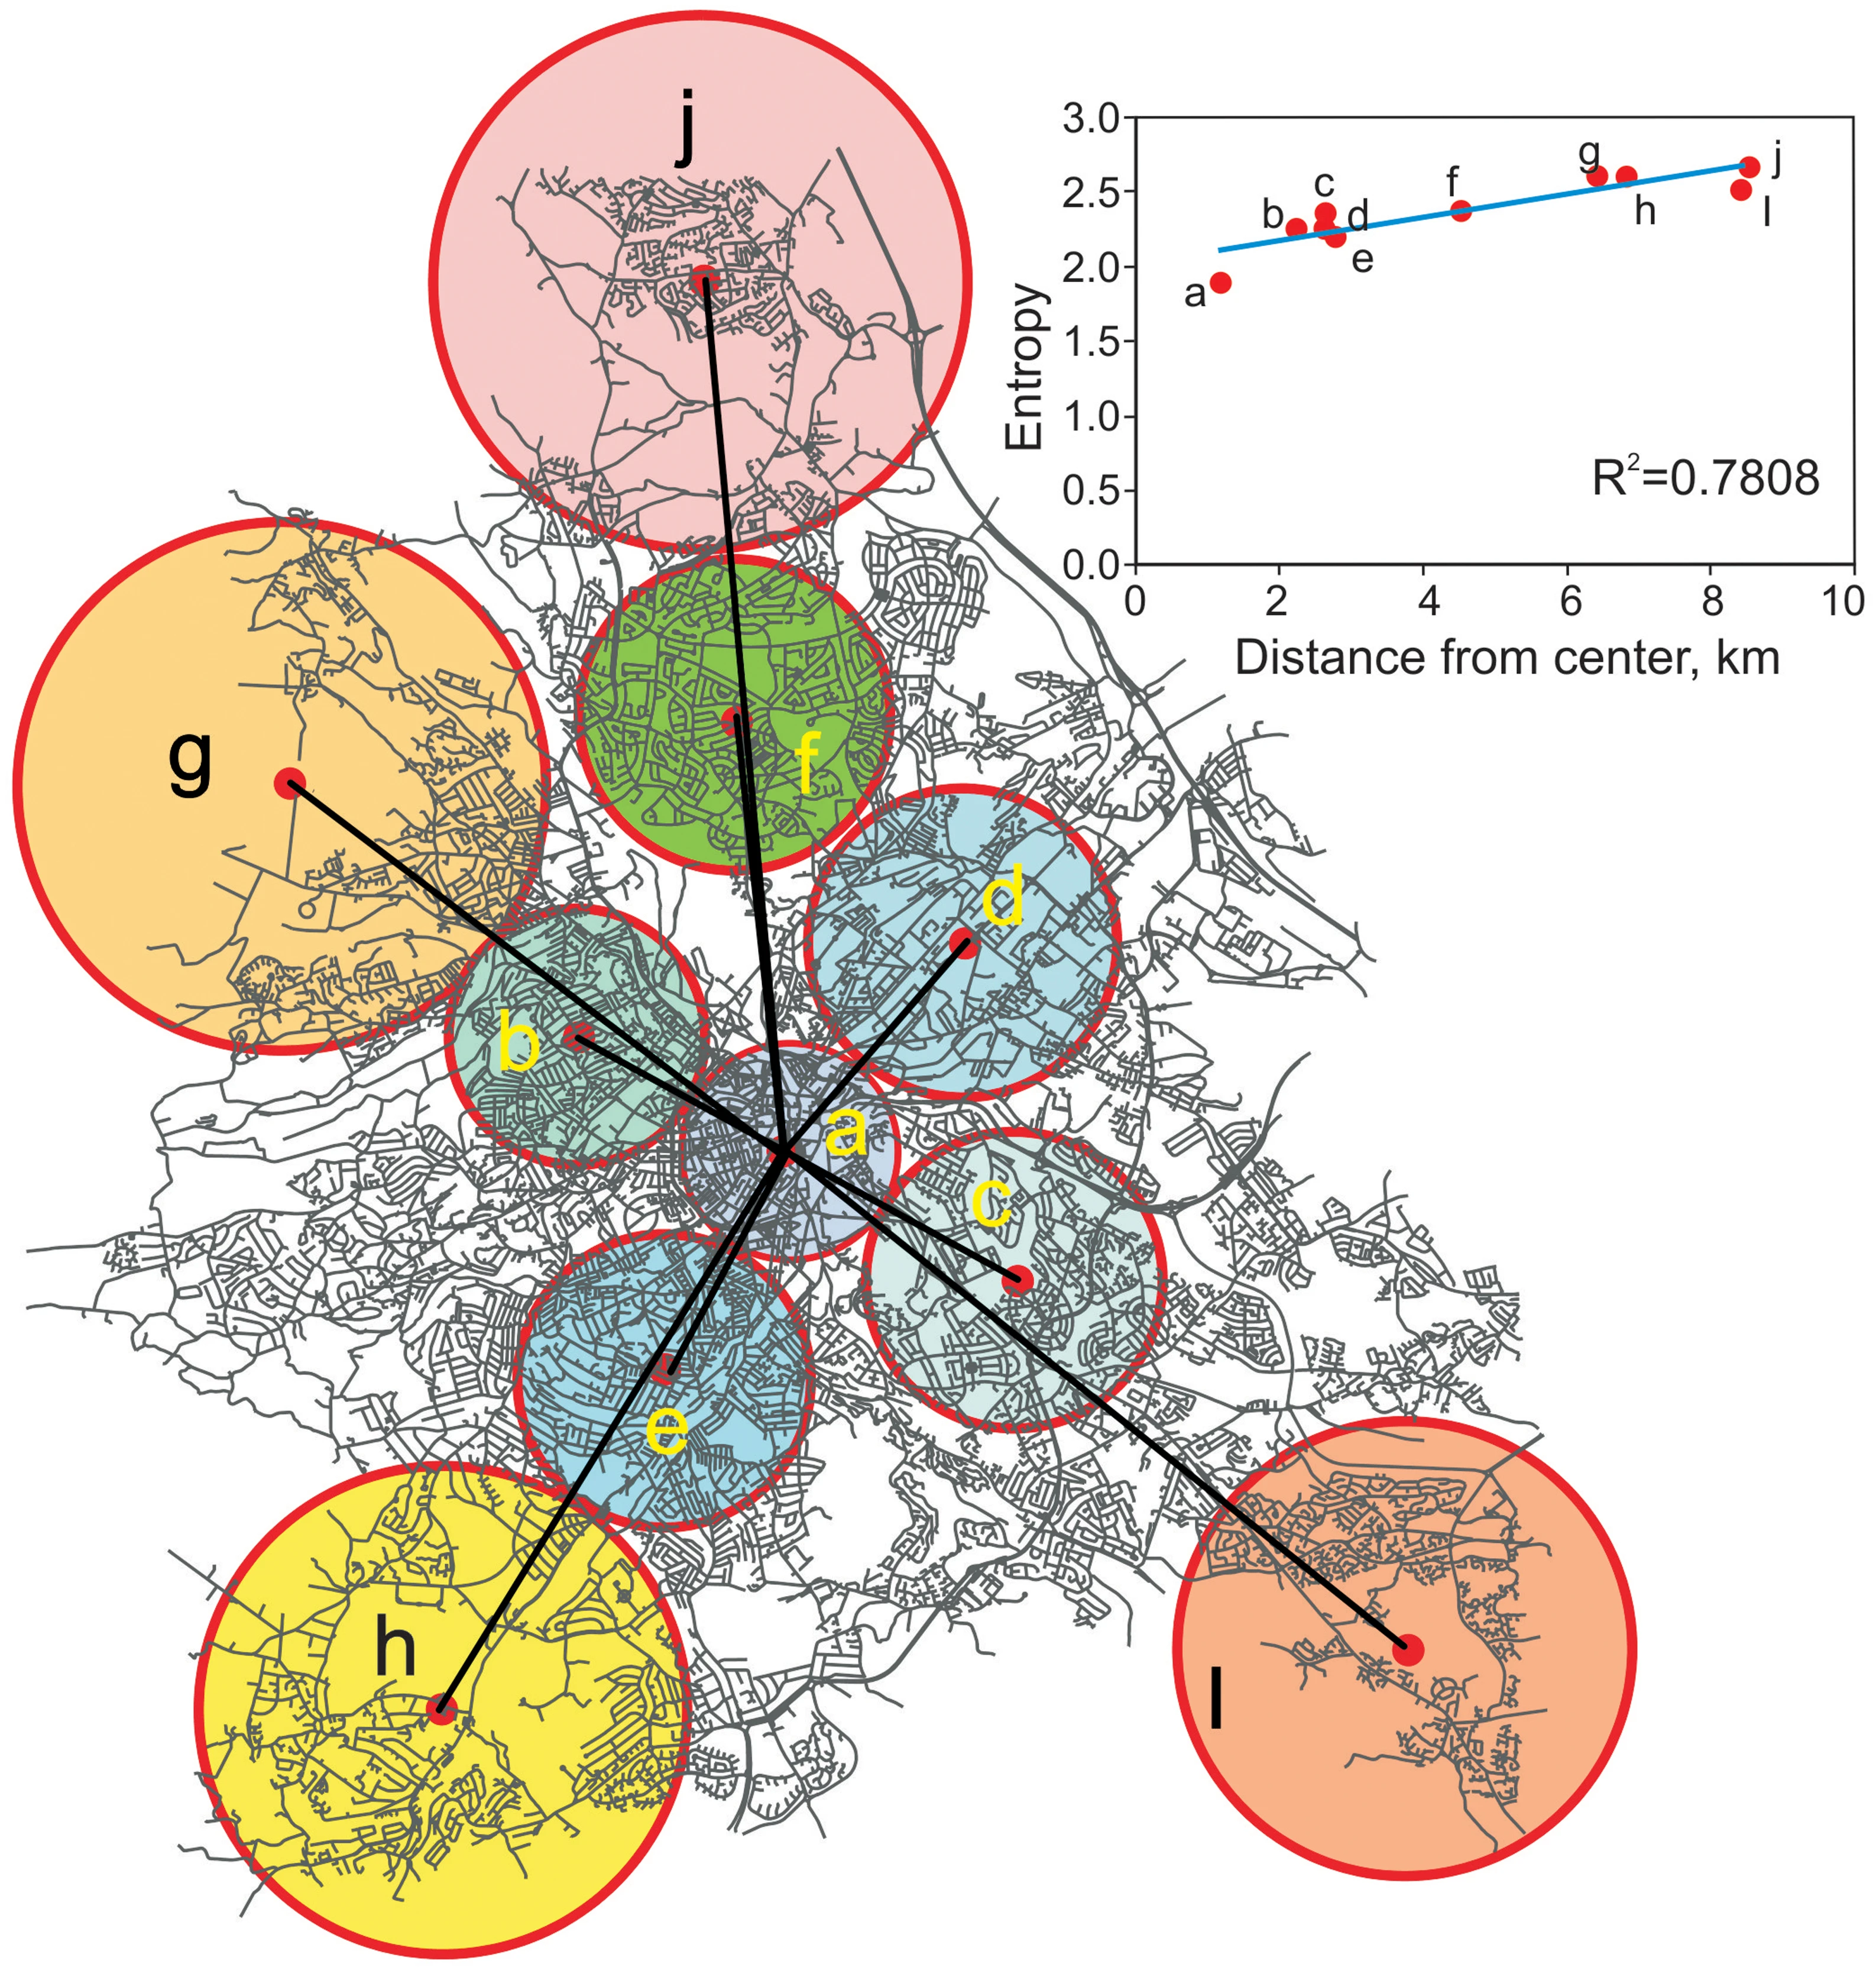
\includegraphics[width=0.8\textwidth]{../variation_length_entropy_Sheffield.png}
    \caption{Variation in length entropy with distance from the centre of the street network of Sheffield. \citet{entropy2020}}
    \label{fig:variation_length_entropy}
\end{figure}

\section{Quantifying Scene Uniqueness}
\citet{entropy2020}, analyzed entropy in urban street networks.
Their findings showed a connection between entropy and urban density, as well as street segment variation.
These measures are useful for assessing how different urban areas develop distinct spatial characteristics.
The study introduced visual representations of orientation histograms, kernel density plots,
and length entropy as tools to capture the unique structure of city layouts, 
which are highly relevant to scene uniqueness, as well as \textit{variation in length entropy 
with distance from the centre of the street network}, which can be used as a separate metric in cases
when the whole area can't be viewed at once - see Figure \ref{fig:variation_length_entropy}.


\section{Research Gaps and Contribution}
Most studies analyze urban spatial order but do not explicitly state what makes a scene stand out visually or structurally. A framework for categorizing distinctive urban scenes is lacking; it is partly addressed by \citet{entropy2020}, but there is still a need for a systematic approach to classify and quantify scene uniqueness.

This research addresses these gaps by developing a methodology to systematically classify geospatially distinctive scenes, quantifying their distribution using entropy and street network metrics, and providing statistical analysis and visualization to understand scene uniqueness better.
